%This fixes a weird error I don't understand
\RequirePackage{ifluatex}
\let\ifluatex\relax

\documentclass[11pt]{article}
\author{Yohan Lefol, Marie Terrien, Alexis Dupis, and Ugo Vidal}

\title{
\textsc{User Guide}\\[2.6cm]
{\LARGE \bfseries CelloMap}
}

\author{
Yohan Lefol
\and 
Alexis Dupis
\and
Ugo Vidal
\and
Marie Terrien
}

\date{
\today
}


\usepackage{hyperref}
\usepackage{graphicx}
\usepackage{apacite}
\usepackage[margin=3cm]{geometry}
\usepackage{comment}
\usepackage[english]{babel}
\usepackage{titlesec}
\usepackage{setspace}

\setcounter{secnumdepth}{4}

\begin{document}
\maketitle
\hrule
\begin{center}

\includegraphics[width = 8cm]{logo-CELLOMET-a.png}
\end{center}

\begin{center}

\includegraphics[width = 7cm]{Logo-Master-GPhy.png}
\end{center}
\thispagestyle{empty}

\doublespacing
\tableofcontents
\singlespacing

\newpage
\section{Introduction \label{intro}}
The non-canonical analysis tool (CelloApp) is a tool with several uses. It's main feature is a non-canonical gene analysis from a gene list. Yet this tool also boasts several other interesting functionalities such a differential expression analysis, customizable MA and Volcano plots which in turn allow to obtain significant gene sets according to a users custom parameters.Additionally, this tool is capable of converting gene symbols to KEGG identifier (type hsa), see \autoref{gene_list_analysis} for more information.
This guide will go over each functionality and explain how to best use CelloApp.

As can be seen in \autoref{fig:main_app_screen}, the application is split into several tabs. The information tab shows two pdf files, the first being this one, and the second being a detailed explanation of the tool and it's components. The last tab 'Citation' is a simple tab which gives the citation information for the use of this tool.This guide will now go over the remaining tabs and explain their uses and how to maneuver them.
\begin{figure}[h!]
\centering
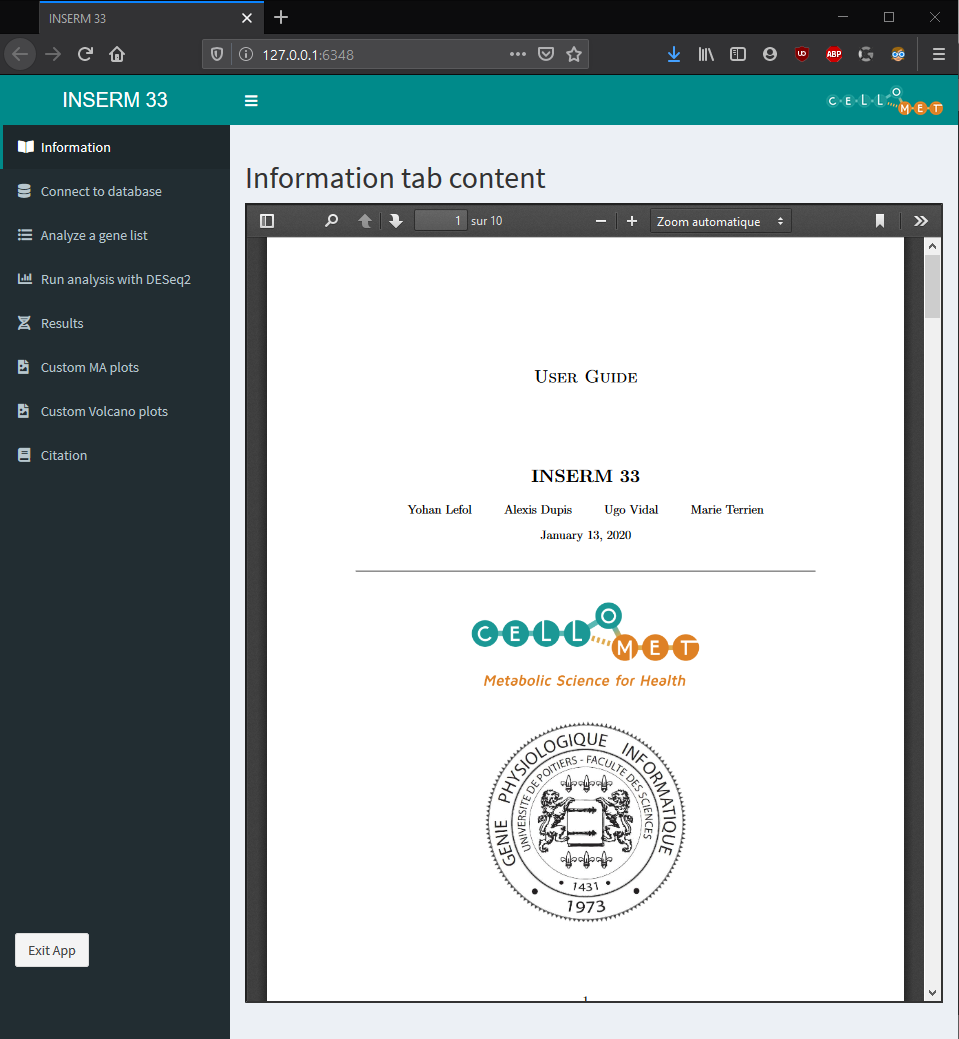
\includegraphics[width=15cm,height=10cm,keepaspectratio]{main_app_screen.png}
\caption{The main tab for the application.}
\label{fig:main_app_screen}
\end{figure}

\section{Installation}
HOW DOES THE INSTALLATION WORK.

\section{Connection to database}
The identification of non-canonical genes is the main aspect of this tool. As the list of non-canonical genes is increasing as discoveries are being made, we could not 'hard code' a list of genes in the program as we wanted to ensure that the search list is being updated without having users re-download the application for each update. Therefore we implemented a database that can be updated by the owners of the tool (Cellomet) and that can be accessed remotely through this application.
In order to establish this connection, a user needs to fill in the small questionnaire as seen in \autoref{fig:connect_DB}, and click the 'Connect to database' button. We created the small questionnaire in order to see the main users of this tool as we intend to keep developing new functionalities and we want these functionalities to be catered to the types of study that require it the most.

\begin{figure}[h!]
\centering
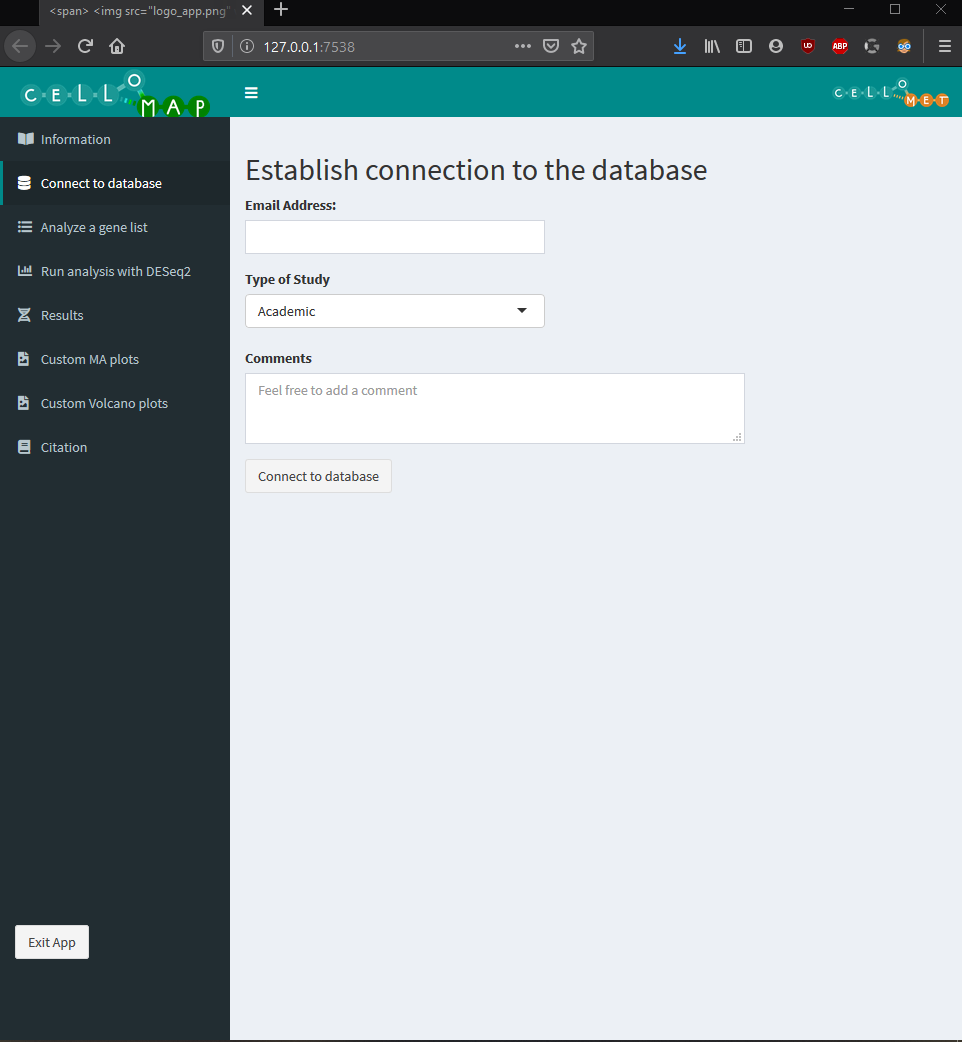
\includegraphics[width=15cm,height=10cm,keepaspectratio]{connect_DB.png}
\caption{The connect to database tab of the application.}
\label{fig:connect_DB}
\end{figure}

The database connection is only necessary if a non-canonical gene analysis is to be performed, either individually or as part of a DESeq2 analysis. If this is not the users intentions, he does not need to establish a connection to the database.

\section{DESeq2 analysis}
DESeq2 is a powerfull tool which allows users to perform differential analyses using RNAseq 'COUNTS' data \cite{love2014moderated}. However this tool requires a very specific data format. This part of the guide will go over the data format necessary to run a DESeq2 analysis, the added parameters specific to this application, and the results that are generated.

\subsection{Tab layout \label{deseq2_layout}}
As seen in \autoref{fig:deseq2_screen}, there are several requirements for the the DESeq2 analysis. First we observe that two csv files are needed, these will be the two files representing the two conditions that will be analyzed. We then observe a small check box which asks if the user want to perform a non-canonical gene analysis. If this box remains checked, the user will have to be connected to the database and the non-canonical gene analysis will be run on the list of significant genes isolated by the DESeq2 analysis (explained below). A user can also select a directory, this will be the folder in which the several DESeq2 results will be saved.
There are then two text boxes which can be customized to be whatever text a user whishes, the content of these text boxes is used to name the files that will be produced by the analysis. Condition 1 represents File 1 and Condition 2 represents File 2.
Lastly there are two check boxes that check if the user would like to create the standard MA and Volcano plots. If checked, two types of each plot will be made, one type with text, and the other without text. The plots generated will be with standard values, however a user will be able to take the differential expression data obtained from the DESeq2 analysis and make his own customized MA and Volcano plots with the custom plot tabs, see \autoref{custom_plots} for more details.

\begin{figure}[h!]
\centering
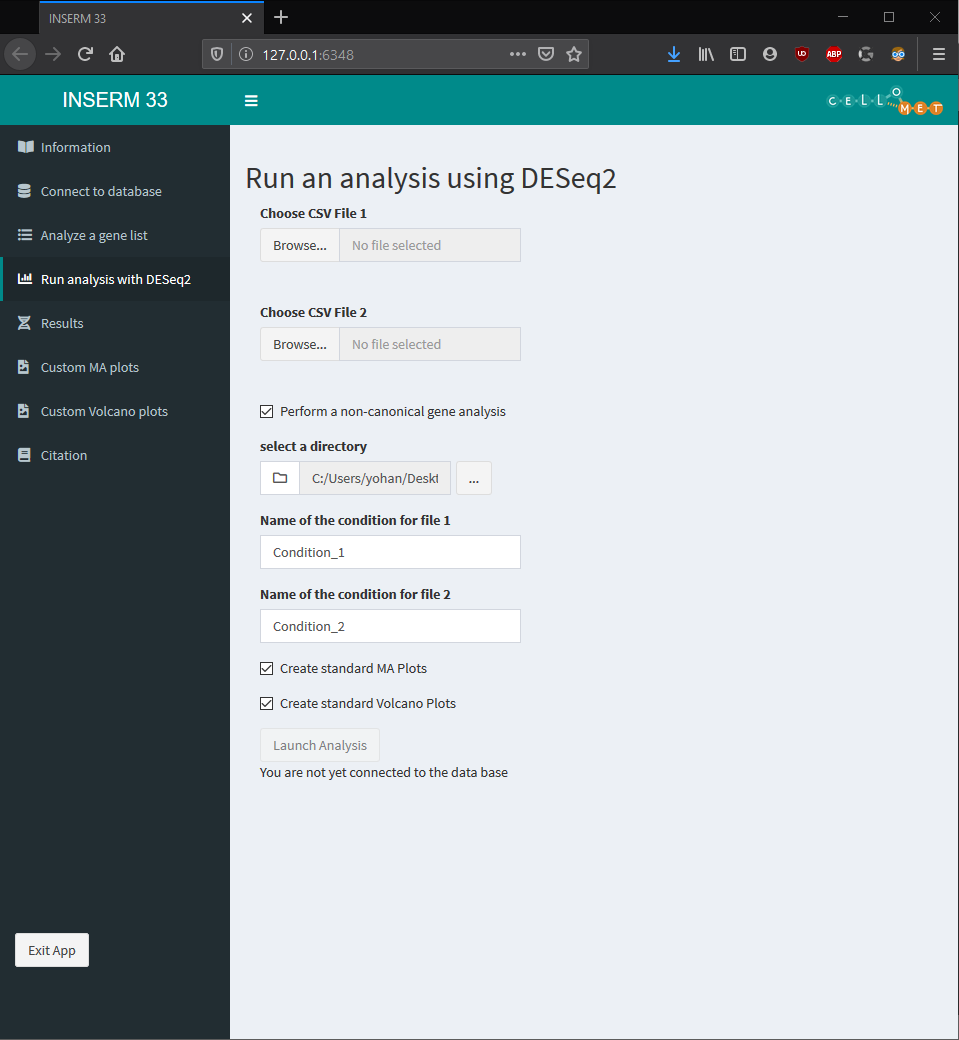
\includegraphics[width=15cm,height=10cm,keepaspectratio]{deseq2_screen.png}
\caption{The main screen for the DESeq2 analysis tab.}
\label{fig:deseq2_screen}
\end{figure}

\subsection{Data format \label{deseq2 data_format}}
As previously stated, DESeq2 requires a rather specific data format. We will be using \autoref{fig:data_format_deseq2} to explain the format.
This format is presented as a CSV file, meaning a comma separated vector, or more simply put, a file in which the different elements/values are separated by a comma.
In order to better explain the data format and what a csv file really is, an excel representation of \autoref{fig:data_format_deseq2} has been created and is shown in \autoref{fig:data_format_deseq2_simplified}

\begin{figure}[h!]
\centering
\fbox{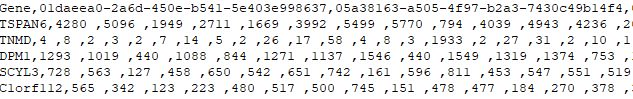
\includegraphics[width=15cm,height=10cm,keepaspectratio]{data_format_deseq2.PNG}}
\caption{The data format for a DESeq2 analysis.}
\label{fig:data_format_deseq2}
\end{figure}

When comparing both \autoref{fig:data_format_deseq2} and \autoref{fig:data_format_deseq2_simplified} we can clearly observe that the commas create the 'separation' of the values. Now we will explain what these values are. 
The first column represents the genes, it is important to note that these genes are in gene symbols and not another type of format such as Ensembl. DESeq2 will perform the analysis regardless of the type of gene name used however \textbf{a non-canonical gene analysis can only be performed with gene symbols}. As such it is advised to use gene symbols in the data in order to fully benefit from this tool. Next we have the other columns which represents the different sequencings. In this example, the second column shows the RNAseq 'COUNTS' results of patient \#1 and the second column shows the same but for patient \#2.
\begin{figure}[h!]
\centering
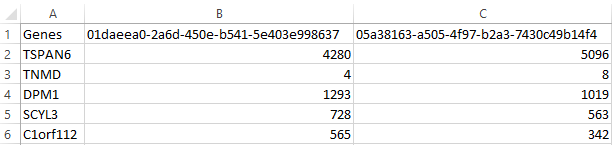
\includegraphics[width=15cm,height=10cm,keepaspectratio]{dese2_excel_data_format.png}
\caption{A simplified view of the DESeq2 data format.}
\label{fig:data_format_deseq2_simplified}
\end{figure}

That's it, that is the data format required. As previously mentioned, two files are necessary, i.e: one file per condition. An easy example to explain this would be the comparative study of young vs old pulmonary cancer patients. In order to do such an analysis, we would have file \#1 contain all of the patients in the 'young' category and file \#2 would contain all the patients of the 'old' category. Of course both files must respect the data format.

\subsection{launching the analysis}
Once all necessary files have been uploaded, a user can click the 'launch analysis' button, at which point a pop-up will appear indicating the the analysis is being performed. This pop-up will lock the application preventing any further use, this is done to avoid the application from crashing if too many actions are performed at once.
It is important to note that a DESeq2 analysis can be very quick just as it may take several hours. The length of the analysis depends on the size of the files used as well as the computing strength of the users computer. If a user is using a old computer, it may be advised to let the computer run the analysis without doing anything else on the side. 
If an error occurs during the analysis, another pop-up will appear stating that there was an error and that the user can read about the error in the error\_log.txt that was created. Using the information from the error log, the user should consult \autoref{common_err} in order to solve the issue.
Once the analysis is done and if no error has occurred, the pop-up message will be replaced by a different pop-up message indicating that the analysis is done, the pop-up message will also remind the user in which files he has stored the results of the analysis.

\subsection{Results obtained}
Several results can be obtained from this analysis, some are obtained regardless of user input, others will only appear if a user has asked for those results to be produced.
\subsubsection{Main results}
A DESeq2 analysis generates three standard results:
\begin{itemize}
\item diffexpr\_results condition\_1 vs condition\_1 .csv\\
A differential expression file
\item condition\_1vscondition\_1\_RESULTS\_VOLCANO.csv\\
A differential expression file for significant genes
\item gene\_list\_ condition\_1 vs condition\_1 \_Most\_Significant.txt\\
A significant gene list
\end{itemize}

It is important to note that the significant genes were obtained by filtering the main differential expression file for standard significance parameters while using a volcano plot to visualize the significant genes. The standard significance algorithm is the following:
\[padj<0.05 \ \&\ abs(log2FoldChange)>2\]
This equation indicates that genes which have a Padj value below 0.05 and a log2FoldChange above 2 or below -2 are considered to be significant. A user can also generate his own list of significant genes by modifying these parameters. This is further explained in \autoref{custom_plots} of this guide.

\subsubsection{Figures generated}
If a user has selected that he wanted standard MA and Volcano plots, there will be four png files in the results folder; Two MA plots, one with text and the other without text, the same applies for the volcano plot.
The plots with texts are much larger in order to accommodate for the additional text besides the points representing significant genes.
If a user wishes to modify these plots and create his own set, it can be easily be done in the custom plot tabs, further explained in \autoref{custom_plots} of this guide.

\subsubsection{Non-canonical gene analysis}
If a user had selected that he wanted a non-canonical gene analysis to be performed, there will three extra text files in the results folder. That is, if any non-canonical genes were found within the significant genes list. The files are the following: 
\begin{itemize}
\item non\_canonic\_results.txt\\
This file will contain the gene symbols and gene names that were found to be non-canonic genes within the significant gene list that was analyzed. The file also contains the non-canonical action and localization of the genes identified
\item canonic\_results.txt\\
Similarly to non-canonic results, however this once contains the canonic action and localization.
\item references.txt\\
Any and all references that were used to identify non-canonical genes and their actions.
\end{itemize}

The results were saved as text files that can easily be read by microsoft excel, or any similar program.
Additionally, results can be viewed immediately in the results tab of the application, see \autoref{res} of this guide for more information.


\section{Gene list analysis \label{gene_list_analysis}}
This tab allows users to perform a non-canonical gene analysis and a gene symbol to hsa identifier conversion with a simple gene list file. The only obligation that this file must respect is that the genes must be in a column with a column header names 'Genes'. If the file entered is correct, a table will appear showing that specific column as seen in \autoref{fig:gene_list_analysis_uploaded}. If this does not occur, a text will appear, stating that a different file should be chosen.
\begin{figure}[h!]
\centering
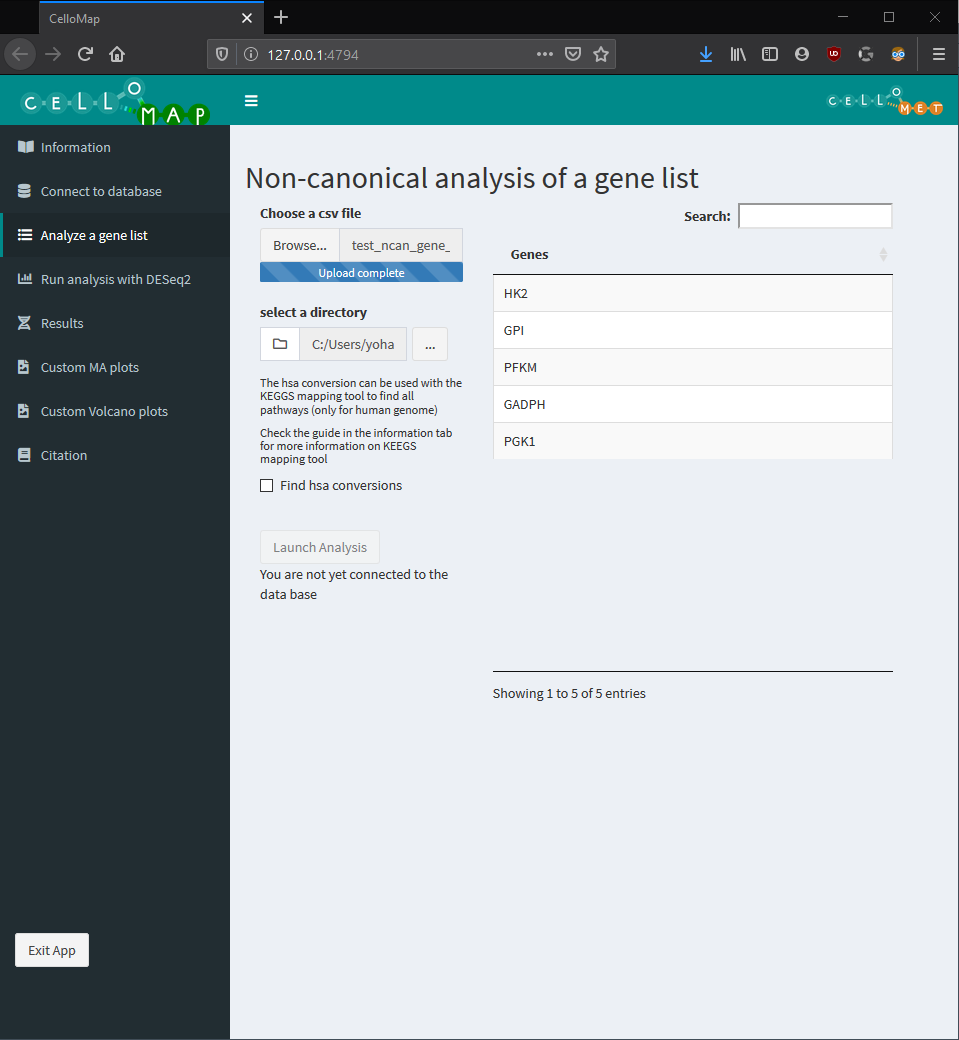
\includegraphics[width=15cm,height=10cm,keepaspectratio]{gene_list_analysis.png}
\caption{The gene list analysis tab once a correct file has been uploaded.}
\label{fig:gene_list_analysis_uploaded}
\end{figure}

Considering that the requirement for this analysis is a single column carrying the name of 'Genes', possible files can be the significant gene list obtained from the DESeq2 analysis, or the significant differential expression results obtained from either the DESeq2 analysis or the downloading of the data from custom plots in \autoref{custom_plots}.
\subsection{KEGG Mapper \label{KEGG Map}}
By checking the 'Find hsa conversions' checkbox in the CelloMap tool, a conversion script will automatically be run along with a non-canonical gene analysis. This conversion will allow users to run a KEGG mapping analysis using the file generated from the conversion.
KEGG Mapper is a mapping tool that will search and find any pathways associated to a list of identifiers provided \cite{kanehisa2019kegg}. It will then allow the user to view every pathway found while highlighting the gene that was in the original list.
To perform the analysis, follow these steps, also seen in \autoref{fig:KEGG_mapper}
\begin{enumerate}
\item Go to the website: \url{https://www.kegg.jp/kegg/tool/map_pathway2.html}
\item Make sure that the search mode is \textbf{Organism-specific} with the letter \textbf{hsa} in the text box
\item Upload the file created by CelloMap, the file will be called \textbf{hsa\_ID.txt} 
\item Launch the analysis and wait a few seconds/minutes
\end{enumerate}

\begin{figure}[h!]
\centering
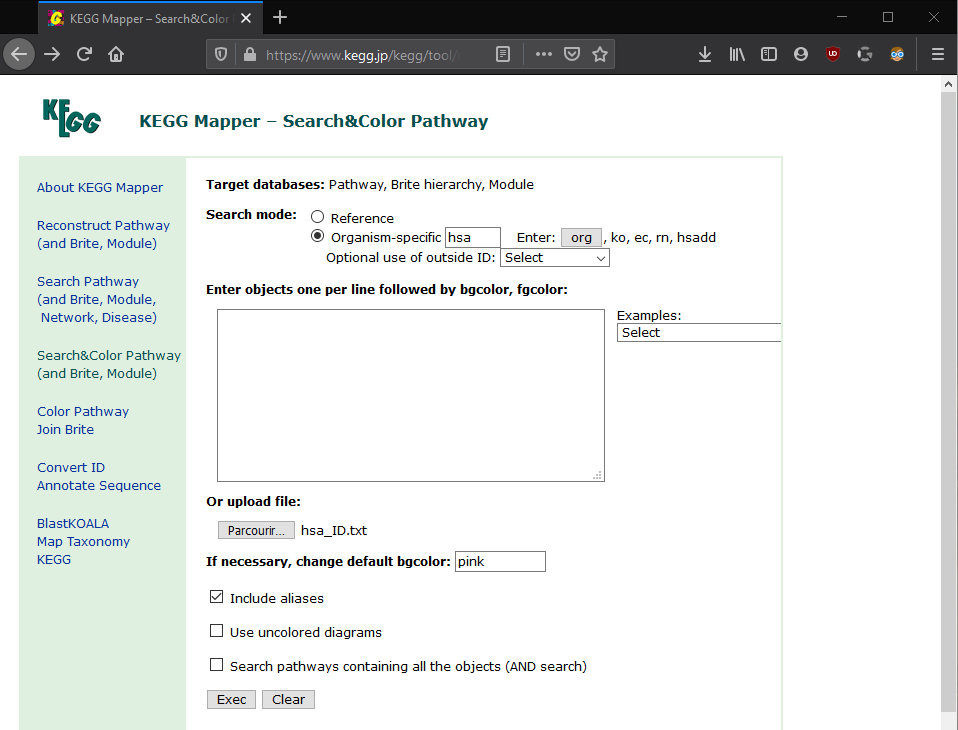
\includegraphics[width=15cm,height=10cm,keepaspectratio]{KEGG_Mapper.png}
\caption{The set-up for the KEGG Mapper tool}
\label{fig:KEGG_mapper}
\end{figure}

\subsection{Metabolic GEne RApid Visualizer (MERAV)\label{MERAV}}
An alternative to the KEGG Mapper is Metabolic GEne RApid Visualizer (MERAV), this tool was designed to analyze \textbf{human} gene expression across a large variety of arrays. All of the arrays were normalized together to generate a gene expression database composed of several types of human tissue \cite{shaul2015merav}.
This tool offers two types of searches:
\begin{enumerate}
\item Search expression levels in one or several genes\\
This search will provide the user with the ability to search the database for the expression of a given gene(s).
\item Search all genes expression levels in one or more cell types\\
This search will provide the user with the ability to search the database for the expression of a given array.
\end{enumerate}

CelloMap creates a significant gene file that can be used with the first type of search, the one relating to finding gene expressions. To perform the search, follow these steps, also seen in \autoref{fig:merav}.
\begin{enumerate}
\item Go to the website: \url{http://merav.wi.mit.edu/}
\item Click the `Search expression levels...' link.
\item Load the gene search box\\
To do this, copy paste all the genes from the significant gene file generated from DESeq2 or the one inputted in the gene list analysis. The main thing to watch out for is to not include the column name 'Genes'. If it is included, it's not a problem, it will simply be considered a gene symbol and will not be found by the search, this will not prevent the tool from searching for the other genes.
\item Set the parameters to your liking
\item If help is required, follow this link: \url{http://merav.wi.mit.edu/help/help.html}
\end{enumerate}

\begin{figure}[h!]
\centering
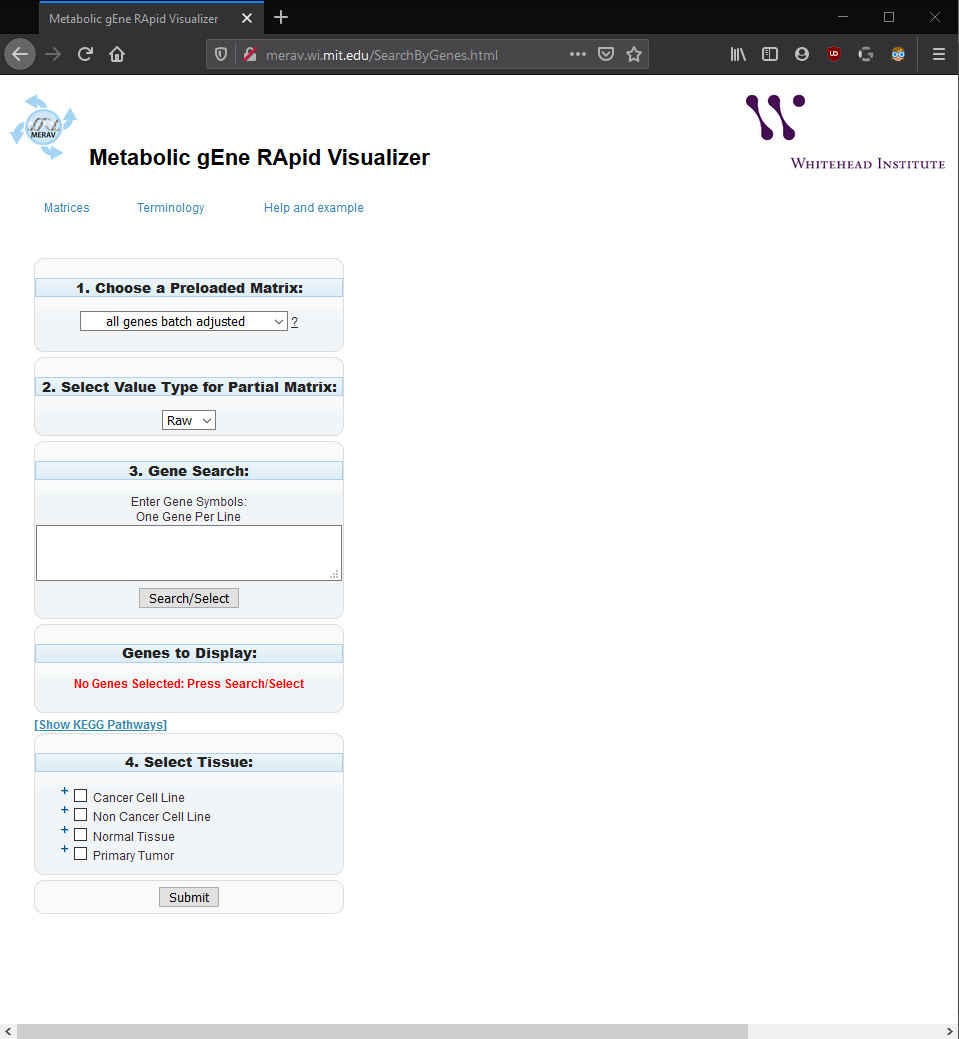
\includegraphics[width=15cm,height=10cm,keepaspectratio]{MERAV.png}
\caption{The set-up for the MERAV search tool}
\label{fig:merav}
\end{figure}

\subsection{Non-canonical gene analysis}
The non-canonical analysis will cross check the provided gene list with our database, and depending on if it finds non-canonical genes within the gene list, three text files will be created.
\begin{enumerate}
\item canonic\_results.txt\\
This file will contain the non-canonical gene symbols and names along with their \textbf{canonical} function and location.
\item non\_canonical\_results.txt\\
This file will contain the non-canonical gene symbols and names along with their \textbf{non-canonical} function and location.
\item references.txt\\
This file will contain the gene symbol and name of non-canonical genes and the references that were used to determine their canonical and non-canonical functions within this database.
\end{enumerate}
Each text file was created with the intention to be read by Microsoft excel. The text files need to be opened in excel and the separator/deliminator must be declared as `Tab'. Once opened, it is recommended to use the `wrap text' and `AutoFit Row Height' in the alignment and cell format sections of excel. This will ensure that the table is legible in excel.
\newpage
\section{Results \label{res}}
The results tab, seen in \autoref{fig:results_tab}, shows the results of a non-canonical gene analysis within the application itself. There isn't much to be said about this tab, it is only for visualization.
Every registered non-canonical genes are registered in a database hosted on Cellomet.com which can be accessed, updated and generally modified by the owner of Cellomet. For any questions regarding the non-canonical genes, their function, localization etc. Please contact Cellomet via their website.

\begin{figure}[h!]
\centering
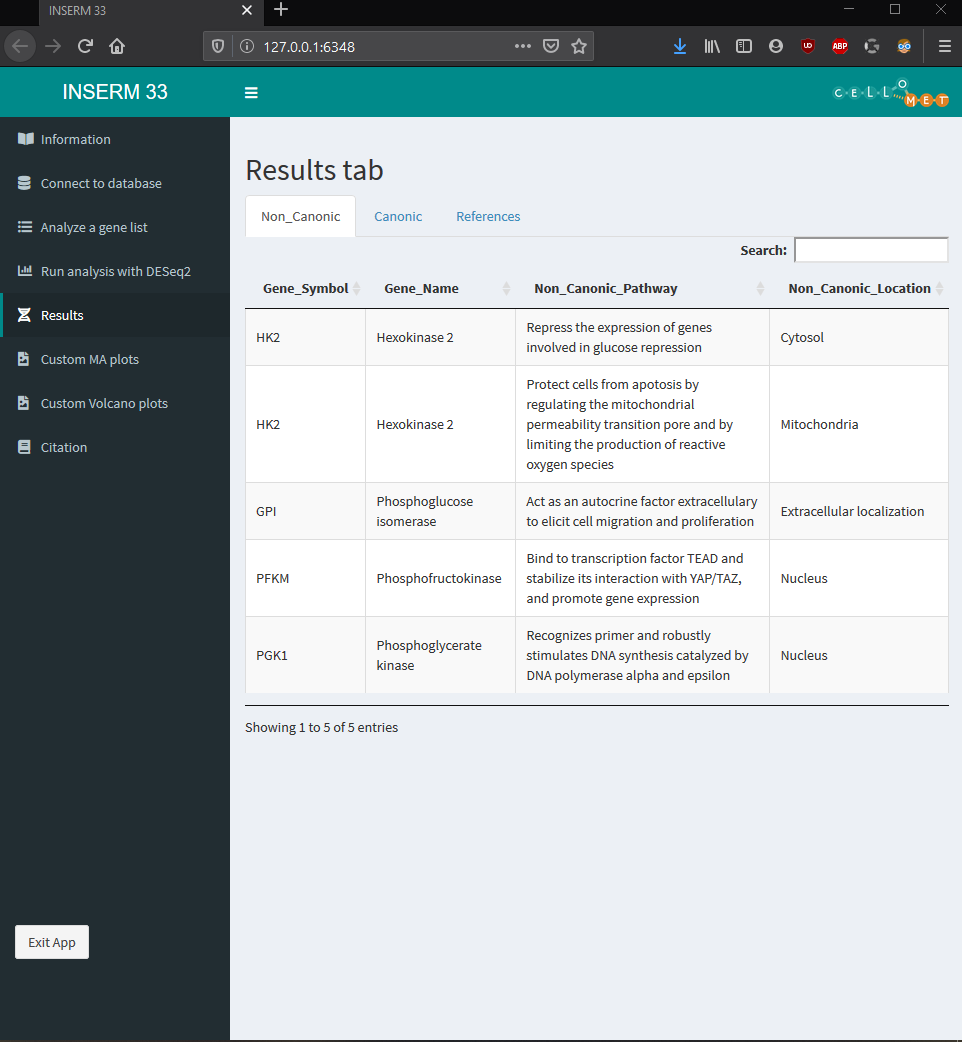
\includegraphics[width=15cm,height=10cm,keepaspectratio]{results_tab.png}
\caption{The results tab after a non canonical gene list analysis.}
\label{fig:results_tab}
\end{figure}

\newpage
\section{Custom MA and Volcano plots \label{custom_plots}}
This application allows users to create their own custom figures, and from these figures, significant gene data can be downloaded. There are two possible figures, MA plots and Volcano plots, each plot type has it's own tab, however they behave very similarly, the volcano plot tab can be seen in \autoref{fig:custom_plots}. 
The main thing to know about these tabs is that a differential expression file is required, like the one obtained from DESeq2 analyses. The columns required are the 'Genes' column, the 'baseMean' column, the log2FoldChange' column, the 'pvalue' column, and the 'padj' column, each written the same way as they are written in the guide. The file must also be a csv file.
Aside that, each element of the different tabs is self explanatory. After each parameter modification, the create plot button needs to be clicked again. When a plot is loading, the rest of the application is locked to prevent the application from crashing due to a potential large number of buffered actions. On every button click the plot must be re loaded from scratch, this factor should be taken into consideration if a user is using a large differential expression files.

\begin{figure}[h!]
\centering
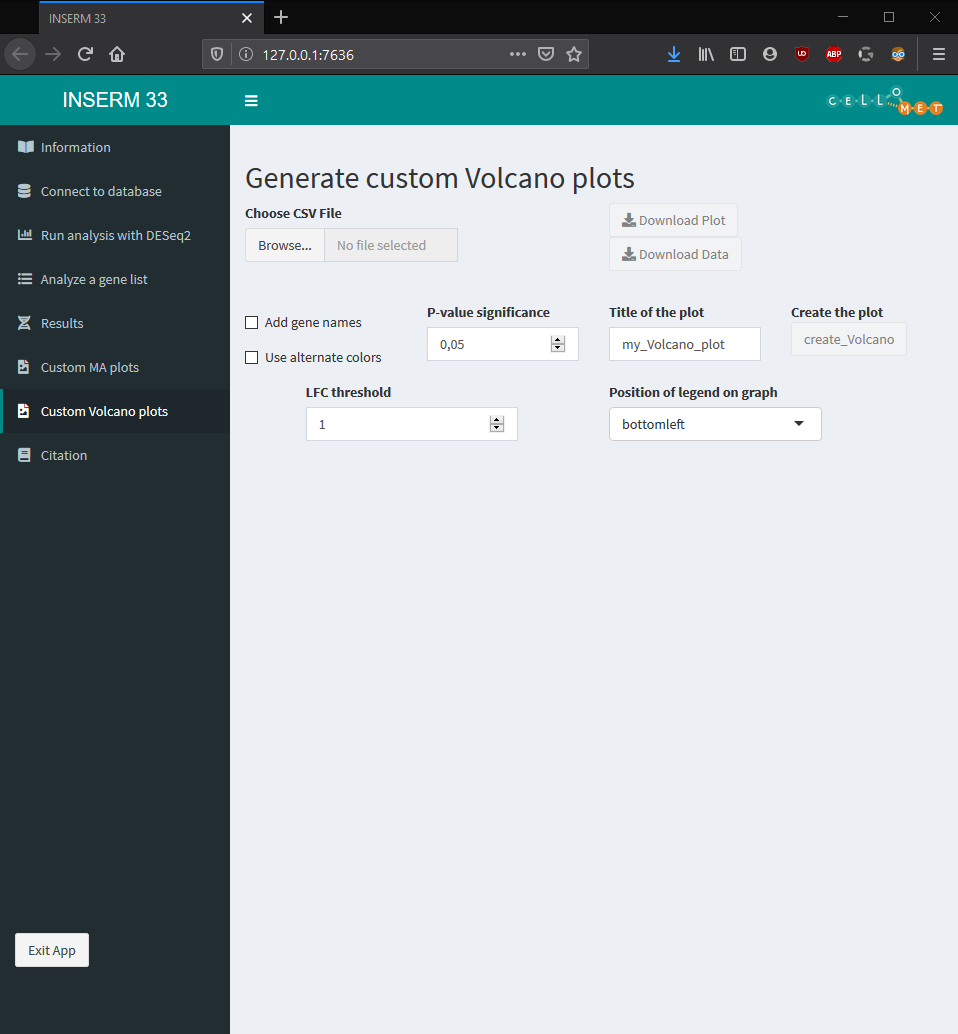
\includegraphics[width=15cm,height=10cm,keepaspectratio]{custom_volcano_tab.png}
\caption{The tab to create a custom volcano plot.}
\label{fig:custom_plots}
\end{figure}


\newpage
\section{Common errors \label{common_err}}
\begin{enumerate}
\item \textbf{Error in DESeqDataSet(se, design = design, ignoreRank): design has a single variable, with all samples having the same value. use instead a design of '~ 1'. estimateSizeFactors, rlog and the VST can then be used}\\
This error may occur when only one condition is named, as well as randomly. It is a simple bug where DESeq2 finds only one variable and thus cannot proceed with its intended process.
To correct this issue, simply try again, make sure that two conditions are names and that both csv files are properly uploaded to the application.
  
\end{enumerate}
\bibliographystyle{apacite}
\bibliography{references}
\end{document}